\begin{center}\section{函数}\label{chapter_function}\end{center}
\subsection{函数相关的定义}
\subsubsection{函数}
设数集$D\in R$的映射
$$f: D\rightarrow R$$
称f为定义在D上的函数,记为
$$y = f(x)\ \{x\in D\}$$
\subsubsection{驻点}
$$Def:\ f'(x)=0$$
\subsubsection{拐点}
$$Def:f''(x)=0\ (\mbox{左右两侧凹凸性改变})$$
\subsubsection{极值点}
$$Def:\mbox{函数}f(x)\ x\in \mathring{U}(x_0),\mbox{包括可导和不可导的点} \begin{cases}
    \mbox{极大值:}f(x)<f(x_0)\\
    \mbox{极小值:}f(x)>f(x_0)
\end{cases}$$
$$x\in \mathring{U}(x_0)\begin{cases}
    f(x)\mbox{可导,}f'(x_0)=0\begin{cases}x_0\mbox{极大值}
        \begin{cases}
            x\in (x_0-\delta ,x_0),f'(x)>0\\
            x\in (x_0 ,x_0+\delta),f'(x)<0
        \end{cases}\\
    x_0\mbox{极小值}\begin{cases}
        x\in (x_0-\delta ,x_0),f'(x)<0\\
        x\in (x_0 ,x_0+\delta),f'(x)>0
        \end{cases}\\
        x_0\mbox{无极值,}x\in \mathring{U}(x_0)\begin{cases}
            f'(x)>0\\
            f'(x)<0
        \end{cases}
    \end{cases}\\
    f(x)\mbox{二阶可导},f'(x_0)=0,f''(x_0)\neq0
    \begin{cases}f''(x)<0\Rightarrow x_0\mbox{极大值}\\
        f''(x)>0\Rightarrow x_0\mbox{极小值}
    \end{cases}
\end{cases}$$
\subsubsection{最值}
$$\mbox{最大值或最小值}\begin{cases}
    \mbox{驻点}\\
    \mbox{端点}
\end{cases}$$
 \subsection{函数的性质}
 \subsubsection{函数的有界性}
 $$f:D\rightarrow R\{D\subset R\}\begin{cases}
    \mbox{有界}\begin{cases}
        \mbox{有上界}\begin{cases}
            \exists k_1,\ \mbox{使}f(x)\leqslant k_1,\ \forall x\in D  
        \end{cases}\\
        \mbox{有下界}\begin{cases}
            \exists k_1,\ \mbox{使}f(x)\geqslant  k_1,\ \forall x\in D  
        \end{cases}
    \end{cases}\\
    \mbox{无界}\begin{cases}
        \mbox{无上界}\begin{cases}
            \forall K_1,\ \exists x\in D\ \mbox{使},\ f(x)\geqslant  k_1
        \end{cases}\\
        \mbox{无下界}\begin{cases}
            \forall K_1,\ \exists x\in D\ \mbox{使},\ f(x)\leqslant  k_1
        \end{cases}
    \end{cases}
 \end{cases}$$
 \subsubsection{函数的单调性与凹凸性}
 $$\mbox{若}\{x_1,x_2\in D\}\ x_1<x_2\Rightarrow \begin{cases}
    f(x_1)<f(x_2)  \mbox{称}f(x)\mbox{在D上单调增加}\\
    f(x_1)>f(x_2)  \mbox{称}f(x)\mbox{在D上单调减少}\\
    f(x_1)\leqslant f(x_2)  \mbox{称}f(x)\mbox{在D上单调非降}\\
    f(x_1)\geqslant f(x_2)  \mbox{称}f(x)\mbox{在D上单调非增}
 \end{cases}$$
 $$\mbox{设$f(x)$在区间I上连续,$\forall x_1,x_2$}\begin{cases}
    f\left(\frac{x_1+x_2}{2}\right)<\frac{f(x_1)+f(x_2)}{2},\mbox{称$f(x)$在I上是向上凹}\\
    f\left(\frac{x_1+x_2}{2}\right)>\frac{f(x_1)+f(x_2)}{2},\mbox{称$f(x)$在I上是向上凸}
 \end{cases}$$
 \begin{align}
    f(x)\mbox{在}\left[a,b\right]\mbox{上连续,在}(a,b)\mbox{内可导}f'(x)\geqslant 0,\mbox{有限个点为0,单调增} \label{monotonous_1}\\
    f(x)\mbox{在}\left[a,b\right]\mbox{上连续,在}(a,b)\mbox{内可导}f'(x)\leqslant 0,\mbox{有限个点为0,单调减} \label{monotonous_2}
 \end{align}
 \begin{align}
    f(x)\mbox{在}\left[a,b\right]\mbox{上连续,在}(a,b)\mbox{内二阶可导}f''(x)\geqslant 0,\mbox{有限个点为0,向上凹} \label{monotonous_3}\\
    f(x)\mbox{在}\left[a,b\right]\mbox{上连续,在}(a,b)\mbox{内二阶可导}f''(x)\leqslant 0,\mbox{有限个点为0,向下凸} \label{monotonous_4}
 \end{align}
\subsubsection{函数的奇偶性}
 $$\forall x\in D\qquad f(-x)=\begin{cases}
    f(x)\qquad &\mbox{偶函数}\\
    -f(x) &\mbox{奇函数}\\
 \end{cases}$$
\begin{align}
    \mbox{奇函数}\times \mbox{奇函数}=\mbox{偶函数}\\
    \mbox{奇函数}\times \mbox{偶函数}=\mbox{奇函数}\\
    \mbox{偶函数}\times \mbox{偶函数}=\mbox{偶函数}
 \end{align}
 \subsubsection{周期性}
 $$Def:\quad f(x+L)=f(x) \{L>0\mbox{常数},\forall x\in D\}\Rightarrow \mbox{$f(x)$为$L$的周期函数}$$
 \subsection{弧}
 \subsubsection{有向曲线弧}
%\noindent\rule[\fill]{\textwidth}{0.4pt}
\begin{minipage}{.5\textwidth}
\begin{center}
			\begin{tikzpicture}[>=latex,scale=2]
		\draw[->](0,0)--(3,0)node[right]{$x$};
		\draw[->](0,0)--(0,2)node[above]{$y$};
		\draw[domain=0:2,samples=1000,red] plot(\x+.5,{\x*\x/3+.5});\node at(2+.5,{2*2/3+.5})[right]{$y=f(x)$};
		\draw[|<->|] (1+.5,{1*1/3+.5})--(1.5+.5,{1.5*1.5/3+.5});\node at(1.3+.3,{1.3*1.3/3+.6})[above]{$\vartriangle s$};
		\draw[dashed](.6,{.1*.1/3+.5})node[above]{$M_0$}--(.6,0)node[below]{$x_0$};
		\draw[dashed](1+.5,{1*1/3+.5})node[above]{$M$}--(1+.5,0)node[below]{$x$};
		\draw[dashed](1.5+.5,{1.5*1.5/3+.5})node[above]{$M'$}--(1.5+.5,0)node[below]{$x+\vartriangle x$};
		\draw[dashed](1+.5,{1*1/3+.5})--(1.25+.5,{1*1/3+.5})--(1.5+.5,{1*1/3+.5});
		\draw[|<->|](1+.5,{1*1/3+.4})--(1.25+.5,{1*1/3+.4})node[below]{$\vartriangle x$}--(1.5+.5,{1*1/3+.4});
		\draw[|<->|](1.5+.6,{1.5*1.5/3+.5})--(1.5+.6,{1.25*1.25/3+.5})node[right]{$\vartriangle y$}--(1.5+.6,{1*1/3+.5});
	\end{tikzpicture}
\end{center}
\end{minipage}
\hfill
\vline
\begin{minipage}{.5\textwidth}
	$$\mbox{基准点}M_0(x_0,f(x_0))$$
	$$\mbox{以$x$增大的方向为正向},\wideparen{M_0M}=S$$
	$$S=S(x),S\mbox{是关于x的单调增加函数}$$
	$$\wideparen{M_0M}\begin{cases}
		\mbox{绝对值为的长度}\\
		\mbox{与曲线正向一致,取正值}\\
		\mbox{与曲线反向一致,取负值}
	\end{cases}$$
\end{minipage}
\subsubsection{弧微分}
\begin{minipage}{.5\textwidth}
\begin{center}
	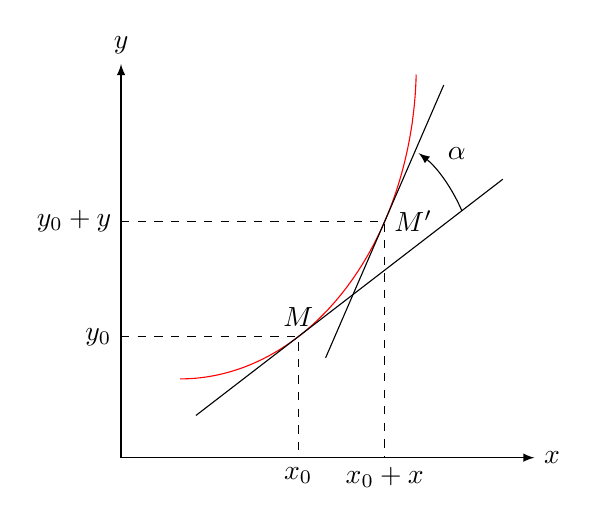
\begin{tikzpicture}[>=latex,yscale=2,xscale=1.5]
		\draw[->](0,0)--(3.5,0)node[right]{$x$};
		\draw[->](0,0)--(0,2.5)node[above]{$y$};
		\draw[domain=0:2,samples=1000,red] plot(\x+.5,{4^.5-(4-\x*\x)^(.5)+.5});
		%\draw[-](.5,2.5)--(1+.5,{4^.5-(4-1*1)^(.5)+.5})node[below]{$M$};
		\draw[dashed] (0,{4^.5-(4-1*1)^(.5)+.5})node[left]{$y_0$}--(1+.5,{4^.5-(4-1*1)^(.5)+.5})node[above]{$M$}--(1+.5,0)node[below]{$x_0$};
		\draw[-]({1+.5-(3^.5)/2},{4^.5-(4-1*1)^(.5)+.5-(1/2)})--(1+.5,{4^.5-(4-1*1)^(.5)+.5})--({1+.5+(3^.5)},{4^.5-(4-1*1)^(.5)+.5+1});
		\draw[->]({1+.5+(3^.5)*.8},{4^.5-(4-1*1)^(.5)+.5+.8}) arc(30:60:1)node[right=7]{$\vartriangle \alpha$};
		%\draw[-](.5,2.5)--(3^.5+.5,{4^.5-(4-3)^(.5)+.5})node[below]{$M'$};
		\draw[dashed](0,{4^.5-(4-3)^(.5)+.5})node[left]{$y_0+\vartriangle y$}--(3^.5+.5,{4^.5-(4-3)^(.5)+.5})node[right]{$M'$}--(3^.5+.5,0)node[below]{$x_0+\vartriangle x$};
		\draw[-]({3^.5+.5-(1/2)},{4^.5-(4-3)^(.5)+.5-(3^.5)/2})--(3^.5+.5,{4^.5-(4-3)^(.5)+.5})--({3^.5+.5+(1/2)},{4^.5-(4-3)^(.5)+.5+(3^.5)/2});
	\end{tikzpicture}
\end{center}
\end{minipage}
\hfill
\vline
\begin{minipage}{.5\textwidth}
	\begin{equation}
		\begin{split}
			ds&=\sqrt{1+(y')^2}dx\\
			&=\sqrt{(dx)^2+(dy)^2}\\
			&=\sqrt{(dx)^2+(f'dx)^2}\label{Arc_differentiation}
		\end{split}
	\end{equation}
	$$\mbox{参数方程}\begin{cases}
		x=\phi(t)\qquad&dx=\phi'(t)dt\\
		y=\psi(t)&dy=\psi'(t)dt
	\end{cases}$$
	$$ds=\sqrt{\left[\phi'(t)\right]^2+\left[\psi'(t)\right]^2}dt$$
\end{minipage}
\subsubsection{曲率}
$$M(x_0,y_0),M'(x_0+\vartriangle x,y_0+\vartriangle y),\vartriangle s =\wideparen{MM'}$$
$$\mbox{曲线上弧的}\begin{cases}
    \mbox{平均曲率:}&\overline{k}=\left|\frac{\vartriangle \alpha}{\vartriangle s}\right|\\
    \mbox{点曲率:}&k=\lim\limits_{\vartriangle s\to 0}\left|\frac{\vartriangle \alpha}{\vartriangle s}\right|=\left|\frac{d\alpha}{ds}\right|
\end{cases}$$
\begin{align}
    \left|\frac{d\alpha}{ds}\right|=\frac{\left|y''\right|}{\left[1+(y')^2\right]^{\frac{3}{2}}}\label{Mean_curvature}
\end{align}
\begin{equation}
    \left|\frac{d\alpha}{ds}\right|\mbox{的参数方程形式\ }\begin{cases}
        x =\phi(t)\\
        y=\psi(t)
    \end{cases}\Rightarrow \left|\frac{d\alpha}{ds}\right|= \frac{\psi''(t)\phi'(t)-\psi'(t)\phi''(t)}{\left\{\left|\psi'(t)\right|^2+\left[\phi'(t)\right]^2\right\}^{\frac{3}{2}}}\label{Point_curvature}
\end{equation}
\subsubsection{曲率圆,曲率半径}
\begin{minipage}{.5\textwidth}
\begin{center}
		\begin{tikzpicture}[>=latex]
		\draw[->](0,0)--(4,0)node[right]{$x$};
		\draw[->](0,0)--(0,4)node[above]{$y$};
		\draw[domain=0:1.5,samples=1000,red] plot(\x+1,{\x*\x+1});
		\draw[] (1,1.5) circle (.5);
		\draw[|<->|,dashed] (1,1.5)--node[above]{r}(1.5,1.5);
	\end{tikzpicture}
\end{center}
\end{minipage}
\hfill
\vline
\begin{minipage}{.5\textwidth}
	$$\mbox{圆的曲率}k=\left|\frac{\vartriangle \alpha}{\vartriangle s}\right|=\left|\frac{\vartriangle \alpha}{r \vartriangle \alpha}\right|=\frac{1}{r}$$
	$$\mbox{曲率半径}r=\frac{1}{k}$$
\end{minipage}